\documentclass{article}
\usepackage[T2A]{fontenc}
\usepackage[utf8]{inputenc}
\usepackage[russian]{babel}
\usepackage{graphicx}
\usepackage[left = 3cm, right = 2cm, top = 2cm]{geometry}
\usepackage{wrapfig}
\usepackage{amsmath}
\usepackage{float}
\graphicspath{ {./images} }

\author{Александр Романов Б01-107}
\date{}
\title{Лабораторная работа №2.2.5\newline Определение вязкости жидкости по скорости истечение через капиляр}
\begin{document}
\maketitle
\newpage
\section{Введение}

\textbf{Цель работы:} 1) определение вязкости воды по измерению объе-
ма жидкости, протекшей через капилляр; 2) определение вязкости
других жидкостей путем сравнения скорости их перетекания со ско-
ростью перетекания воды.\\
\textbf{В работе используются:} сосуд Мариотта; капиллярная трубка;
мензурка; секундомер; стакан; микроскоп на стойке.

\section{Работа}
\subsection{A. Измерение вязкости воды}
Запишем параметры установки:

\begin{figure}[H]
    \centering
    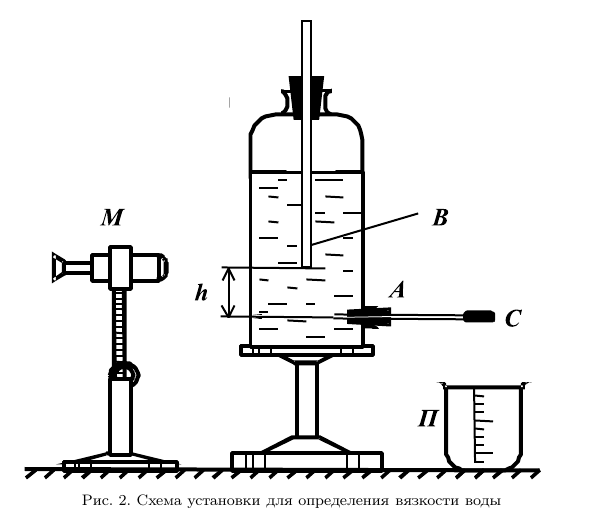
\includegraphics[width=0.6\textwidth]{device.png}
\end{figure}

\begin{figure}[H]
    \centering
    \begin{tabular}{|c|c|}
        \hline
        Длина капилярa A, мм&Диаметр капиляра A, мм\\\hline
        131&9\\\hline
    \end{tabular}
\end{figure}

\begin{enumerate}
    \item 
Снимем пробку С и, дождавшись первых пузырьков на нижнем конце трубки B, начнём измерения 
расхода воды.
Два раза измерим время за которое мензурка заполняется на 25 мл (185 и 180 с). Мы 
понимаем, что скорость истечения не зависит от уровня воды в сосуде. Измерения проводились при 
$h = 85 \text{мм}$.

    \item
Приступим к основной серии измерений. Мы будем менять глубину погружения трубки В и измерять 
время, за которое через капиляр вытечет 20 мл воды. Результаты измерений занесём в таблицу:

\begin{figure}[H]
    \centering
    \begin{tabular}{|c|c|c|c|c|c|}
        \hline
        $h$, мм&29&38&44&57&62\\\hline
        $t_{\text{зап}}$, с&576&383&327&248&213\\\hline
    \end{tabular}
\end{figure}

Вычислив расход воды по формуле:
\[ Q = \frac{V}{t_{\text{зап}}} \]
Получим слудующие данные:

\begin{figure}[H]
    \centering
    \begin{tabular}{|c|c|c|c|c|c|}
        \hline
        $h$, мм&29&38&44&57&62\\\hline
        $Q$, $\frac{\text{мл}}{c}$&0.035&0.052&0.061&0.081&0.094\\\hline
        $Re$&2.5&3.69&4.3&5.73&6.65\\\hline
        $a$, мм&2.25&3.32&3.87&5.16&5.98\\\hline
    \end{tabular}
\end{figure}
Где $a$ - это расстояние пройдя которое в капиляре установиться ламинарное течении.
В его вычислении мы использовали формулу:
\[ a = 0.2R\cdot Re = 0.2R\cdot\frac{QR\rho}{S\eta}\]

Изобразив $Q(h)$ на графике:

\begin{figure}[H]
    \centering
    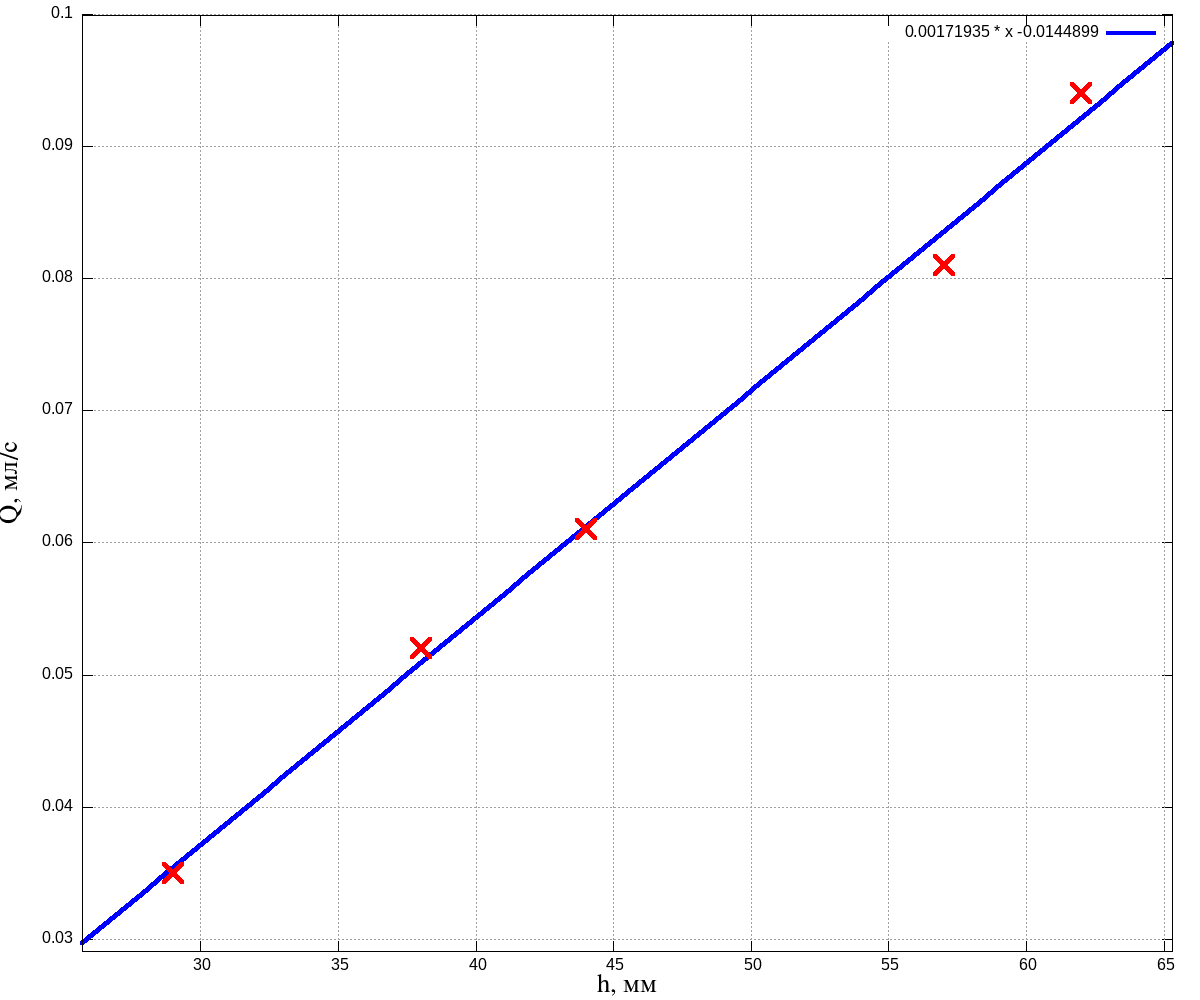
\includegraphics[width=0.8\textwidth]{A.png}
\end{figure}

Полчуена зависимость вида ($y = kx + b$):\\
$k = 0.0017 \pm 5.56979\cdot10^{-5} \frac{\text{мл}}{\text{c}\cdot \text{мм}}$;

$b = -0.0144 \pm 0.0007 \frac{\text{мл}}{\text{с}}$
По углу наклона графика определим вязкость воды:
\[ \eta = \frac{\pi R^4\rho g}{8lQ'(h)} = 0.0072 \text{П} \]

\end{enumerate}
\subsection{B. Измерение вязкости раствора глицерина вискозометром Оствальда}

Будем измерять время протекания между отметками "1" и "0" Вискозометра различных жидкостей. 
Результаты измерений сведём в таблицу:

\begin{figure}[H]
    \centering
    \begin{tabular}{|c|c|c|c|c|c|c|c|}
    \hline
        Номер опыта&1&2&3&4&5&Среднее значение&погрешность\\ \hline
        $t$ воды, с& 5,91 & 5,87 & 5,84 & 5,89 & 6,09 & 5,92 & 0.039\\ \hline
        $t$ глицерина 10\%, с& 8,32 & 8,36 & 8,33 & 8,68 & 8,86 & 8,51 & 0.242\\ \hline
        $t$ глицерина 20\%, с& 10,72 & 11,35 & 10,65 & 10,79 & 11,17 & 10,94 & 0.376\\ \hline
        $t$ глицерина 30\%, с& 15,15 & 15,18 & 15,49 & 15,19 & 15,08 & 15,2 & 0.099\\ \hline
    \end{tabular}
\end{figure}

Вычислим коэффициенты вязкости растворов по формуле:
\[ \eta_x = \eta_0\frac{\rho_x}{\rho_0}\frac{t_x}{t_0}\]

Получим значения:

\begin{figure}[H]
    \centering
    \begin{tabular}{|c|c|}
        \hline
        Глицерин, \%&$\eta$, cП\\ \hline
        10&1.1\\ \hline
        20&1.4\\ \hline
        30&1.97\\ \hline 
    \end{tabular}
\end{figure}

Эти значения достаточно точно совпдают с табличными:

\begin{figure}[H]
    \centering
    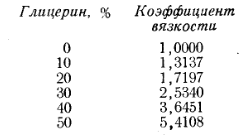
\includegraphics[width=0.3\textwidth]{table_data.png}
\end{figure}

\section{Выводы}
\begin{enumerate}
    \item 
В данной работе мы определили коэффициент вязкости воды при температруе около 293 K
по скорости протекания через капиляр при постоянном давлении. Полученное
значение (0.0072 П) довольно неплохо совпадает с табличным (0.011 П)
    \item 
Мы также определили коэффициенты вязкости воднфх растворов глицерина пользуясь 
вискозиметром Оствальда. Полученные значения также совпадают с табличными весьма точно.
\end{enumerate}






\end{document}